% Chapter 4

\chapter{The Study of spatial-temporal data and its Applications} % Chapter title

\label{ch:study} % For referencing the chapter elsewhere, use \autoref{ch:name} 

%----------------------------------------------------------------------------------------
\section{Point-based Irrigation Water Usage Decision Support System}
A point-based intelligent system is developed as a proof-of-concept for using Machine Learning in the field of agriculture decision support system. This system integrates the use of a server-end computing cloud that access and process multiple data sources, a modern web portal that facilitates 24/7 data access via wireless and an android application that provides the capability of instant notification and real-time access to an intuitive graphic decision support system.
%------------------------------
\subsection{Scope and Requirements}
\begin{itemize}
  \item Purpose: Proof of concept product
  \item Customers: Anyone who is willing to access to irrigation water usage information, especially the farmers in regional areas
  \item Functionality: The system should be fully functional despite being a prototype. 
  \item Connectivity: While in trial period, the system should be operational at 24/7, with automated daily database update on the computing cloud. The data transmitted between the server and the client should be compact, via a human-readable text-based format, namely \ac{json}. 
  \item Operating System: Server-end program is to be operated on both Windows and Linux OS; Client-end app is to be operated in Android 2.2+
  \item Programming language: A cross-platform programming language should be used, namely Java.
  \item User Interface: The client-end app should have a map with relevant information overlays, namely Google Maps. The client-end app should have an intuitive indicator system.
  \item Error handling level: Low. Operational is the minimum requirement for the system.
\end{itemize}
%------------------------------
\subsection{Methodology}
\subsubsection{Knowledge integration on computing cloud}
The workflow of the server-end process is illustrated as in \autoref{fig:mobilecloudschematic}. Based on any given location information (latitude and longitude) the nearest available BOM weather station was selected based on geographical distance. A SILO data file was downloaded and processed for the chosen station. The nearest available CosmOz data was also downloaded for the selected station. The AWAP database was connected through a secured FTP server and grid files were downloaded locally. For the same location a pixel position was derived on the daily continental AWAP gridded data and time series were extracted for individual variable for a given time frame.\\
\newline
The work flow is implemented using Java as the programming language, namely the package \emph{au.csiro.iekbase.cosmoz}, \emph{au.csiro.iekbase.water} and \emph{au.csiro.iekbase.wrapper}. Where package \emph{cosmoz} facilitates download and access of the data from remote servers, package \emph{water} formulates the calculation of water balance indices and implements the machine learning process, and package \emph{wrapper} constitutes the automation or bulk process for all supported sensor stations in Australia. A Linux bash script is scheduled to be run at 6am \ac{aest} daily to ensure that the entire database is up-to-date with remote servers.\\
	\begin{figure}[bth] 
	\begin{center}
	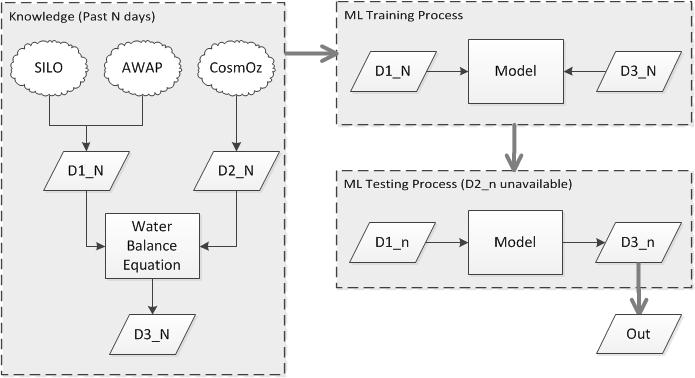
\includegraphics[width=.95\linewidth]{gfx/Sch_mlp2}
	\end{center}
	\caption{Workflow of server-end process for point-based study}
	\label{fig:mobilecloudschematic}
	\end{figure}
\newline
Referring to the water balance model outlined in \autoref{subsection:implementwaterbalance}. A conditional rule is complemented as shown below such that the water balance of each time frame is labelled either class 1, indicating surplus water in the soil, or class 2, indicating deficit water in the soil.
\begin{align}
\Delta\langle WB\rangle &= \langle P\rangle - \langle ET\rangle-\langle Q\rangle-\langle R\rangle-\Delta \langle S\rangle
\end{align}
\begin{quote}
if $\Delta\langle WB\rangle >0$:\hspace{1cm}Indicator = $C_1$\\
if $\Delta\langle WB\rangle <0$:\hspace{1cm}Indicator = $C_2$\\
if $\Delta\langle WB\rangle =0$:\hspace{1cm}Ideal balance situation
\end{quote}
\subsubsection{Linear Discriminant Clustering}
\ac{lda} and the related Fisher's linear discriminant are methods used in statistics, pattern recognition and machine learning to find a linear combination of features, which characterizes or separates two or more classes of objects or events. The resulting combination may be used as a linear classifier or, more commonly, for dimensionality reduction before later classification.\\
\newline
Based on the hydrological water balance calculation, a
daily water requirement status indicator was generated and used as class boundaries between two types of irrigation scenarios, namely, "Extra irrigation required'' and ``No extra irrigation required''.Default \ac{lda} (D-LDA) was applied to cluster the historical sensory data according to these two categories to create a water availability decision support knowledge mapping. 

\subsubsection{Case study: Daly River}
A case study is conducted to analyze the validity of the proposed approach. Data from Daly River ($14.2^\circ S, 131.4^\circ E$) was integrated and processed for this study. This location was selected to induce significant data variance in the generalization experiments as geographically they are quite different in nature. Daly River is a tropical savannah. The time period of the experiment was 01/01/2011 �C 31/12/2012. The study was conducted on a daily time frame.\\
\newline
A time series was created to represent the variance of irrigation water requirement indicator over two complete years.\\
\newline
\autoref{fig:dalyindicator} shows the irrigation indicator profile whereas \autoref{fig:dalyclusters} shows the unsupervised cluster map based on D-LDA for irrigation water usage for the case study of Daly River.\\
\begin{figure}[hbt]
\myfloatalign 
\subfloat[{Daly River irrigation indicator profile}]
{\label{fig:dalyindicator}
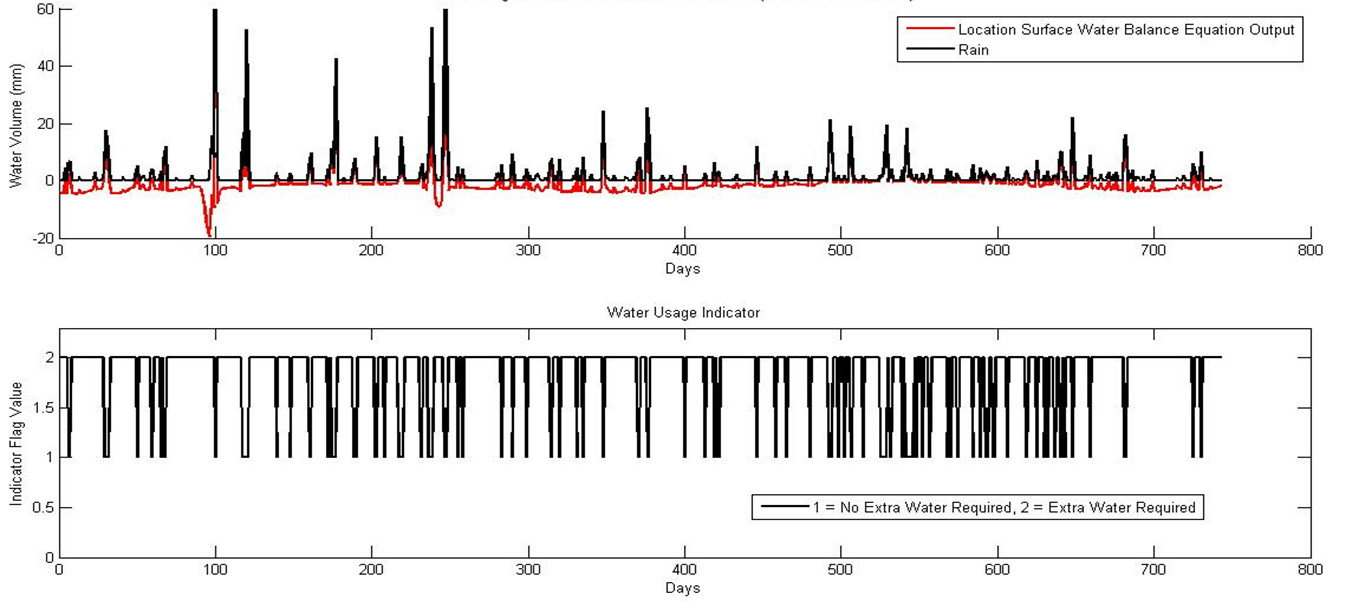
\includegraphics[width=.95\linewidth]{gfx/dalyindicator}}\\
\subfloat[{Daly River irrigation water usage cluster map}] 
{\label{fig:dalyclusters}
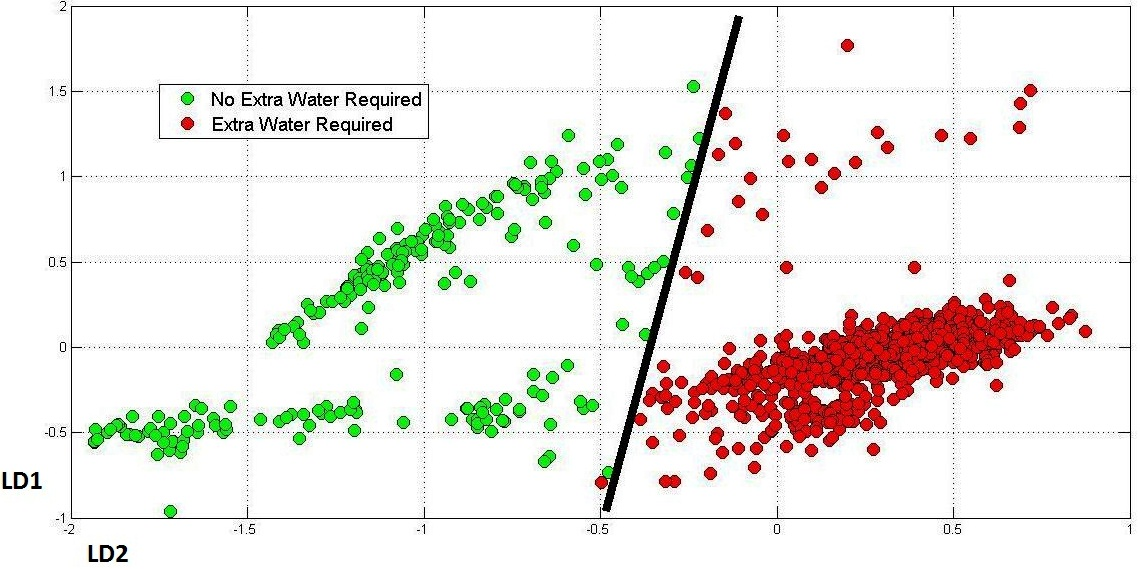
\includegraphics[width=.95\linewidth]{gfx/dalyclusters}}
\caption{Daly River Irrigation Profile and Cluster Analysis}
\label{fig:dalyfigures}
\end{figure}
\newline
Overall accuracy of the machine learning framework was measured using the two year long historical data set. 50\% of the historical data set was used for creating the two clusters based unsupervised dynamic knowledge map representing two classes. The remaining 50\% was used to verify the accuracy of the mapping. The result performance was 92.3\% overall accuracy with 93\% sensitivity and 94\% specificity.
\subsubsection{Web Interface}
\label{webinterface}
The web interface is developed to be operational 24/7 when in trial period, it utilise the use of Play 2.0 framework\citep{play2014}. Play 2.0 framework is a light-weight, stateless and web-friendly architecture that uses Java or Scala as the programming language. Its support for Java language makes it suitable for the application as there would be minimum amount of effort to bridge between the other server-end programs and the web interface. The web interface provides a specifically defined JSON format data via HTML method, the JSON format contains information on application version, date of last update, available locations, the latitude, longitude, elevation and other geographic information of each location and the irrigation water usage indicator label for each location. A sample can be found in the \autoref{JSONsample}.

\subsubsection{Android Application Development}
The Android application is developed as a fully-functional proof of concept product. It is developed to be operational on any device that supports Android 2.2+, it uses minimal amount of internal space for application installation, it retrieves data from the web portal via the specifically defined JSON format as explained in \autoref{webinterface}.\\
\newline
\autoref{fig:androidflow} illustrates the recommended application flow, which can be simplified as a two stage process: Stage 1, Google Maps overview of all available stations in Australia as an overlay layer representation; Stage 2, traffic light style indication of irrigation water balance status of the user-specified station. As shown in \autoref{fig:androidmenu} the user is able to locate himself/herself on the Google Map by clicking on the ``Location'' button in the menu bar at the bottom of the screen, the user is also able to switch between satellite view and normal view of the map depending on personal preference.
\begin{figure}[hbt]
\myfloatalign 
\subfloat[{Stage 1: Overview}]
{\label{fig:androidstage1}
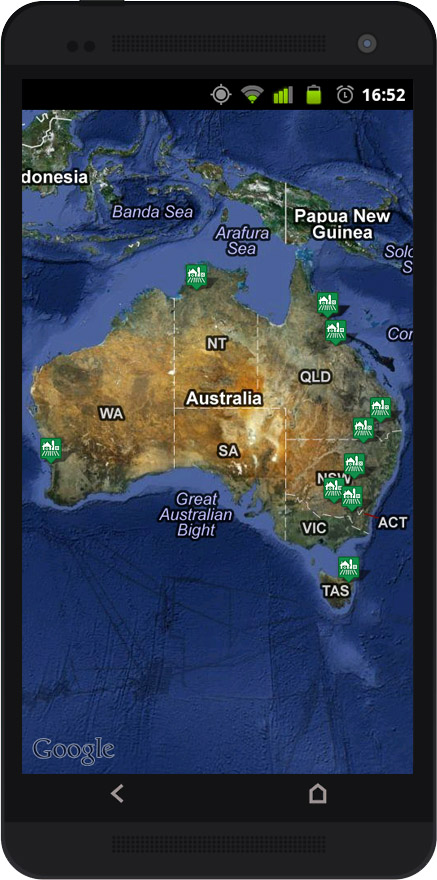
\includegraphics[width=.30\linewidth]{gfx/androidstage1}}\quad
\subfloat[{Stage 2: Detailed view}] 
{\label{fig:androidstage2}
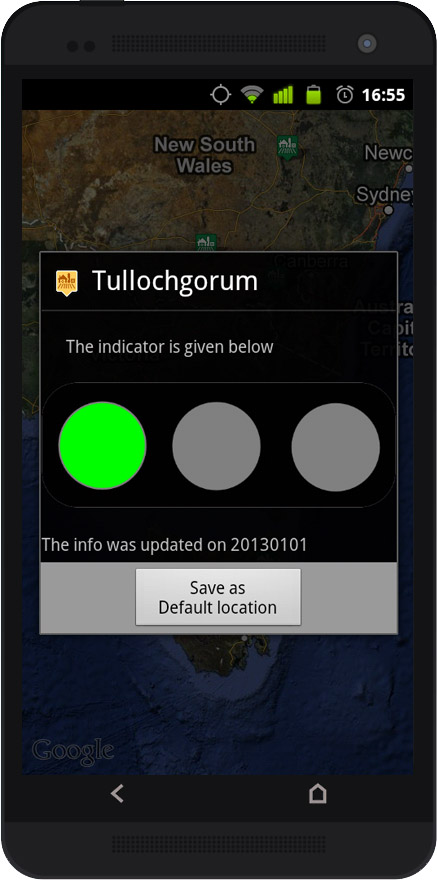
\includegraphics[width=.30\linewidth]{gfx/androidstage2}}\quad
\subfloat[{(Optional) Menu pop-up}] 
{\label{fig:androidmenu}
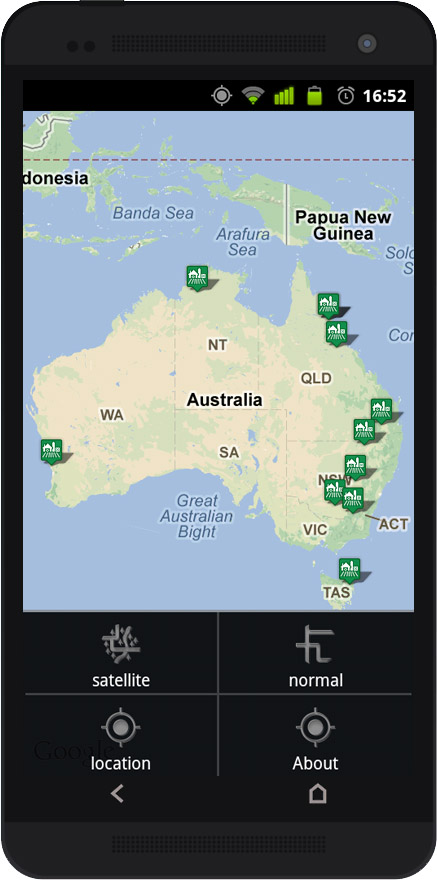
\includegraphics[width=.30\linewidth]{gfx/androidmenu}}
\caption{Android Application Work Flow Illustration}
\label{fig:androidflow}
\end{figure}
\subsection{Limitations of point-based study}
There are a few limitations and drawbacks with this proof-of-concept study.\\
\newline
First of all, a single point trained model is very specific, which means that it cannot be generalised for any other locations. Therefore, it is incapable to choose any arbitrary location and retrieve the information of that location using this approach. Secondly, the binary classification in this study can be improved by introducing more variations of classes. Thirdly, due to the dependency on CosmOz and SILO data, the data can only be available at where both sensor stations are present, which has a very limited number. Fourthly, the data sources used for this study are entirely provided by facilities that have association with Australian Federal Government more or less, therefore the data could have dependencies on each other.
%---------------------------------------
\section{Area-wise water balance study}
The preliminary analysis of the data via a point-based method has proved to have certain validity and usefulness as a decision support tool. To further extend the research, an area-wise water balance study which utilise the exact water balance modelling method is proposed and conducted to validate for viability and accuracy.
\subsection{Implementation}
\autoref{fig:areawisephase1} shows how the data are stored and pre-processed prior to conducting the machine learning analytic procedures. Firstly, the time range of interest is defined, of which individual weekly folders are created to store the data. Secondly, a region of interest is defined with the following parameters: the latitude and longitude of a centre point, the width and the height of a rectangle that is centred by that point. Thirdly, for each week the AWAP and MODIS VI data are extracted for that rectangle region of interest, which has a 5km/pixel and 250m/pixel resolution respectively. Lastly, the water balance index as explained in \autoref{eq:wbsimple} is calculated at the same spatial resolution as the AWAP data, as the ground truth for the later stage analysis.\\
	\begin{figure}[bth] 
	\begin{center}
	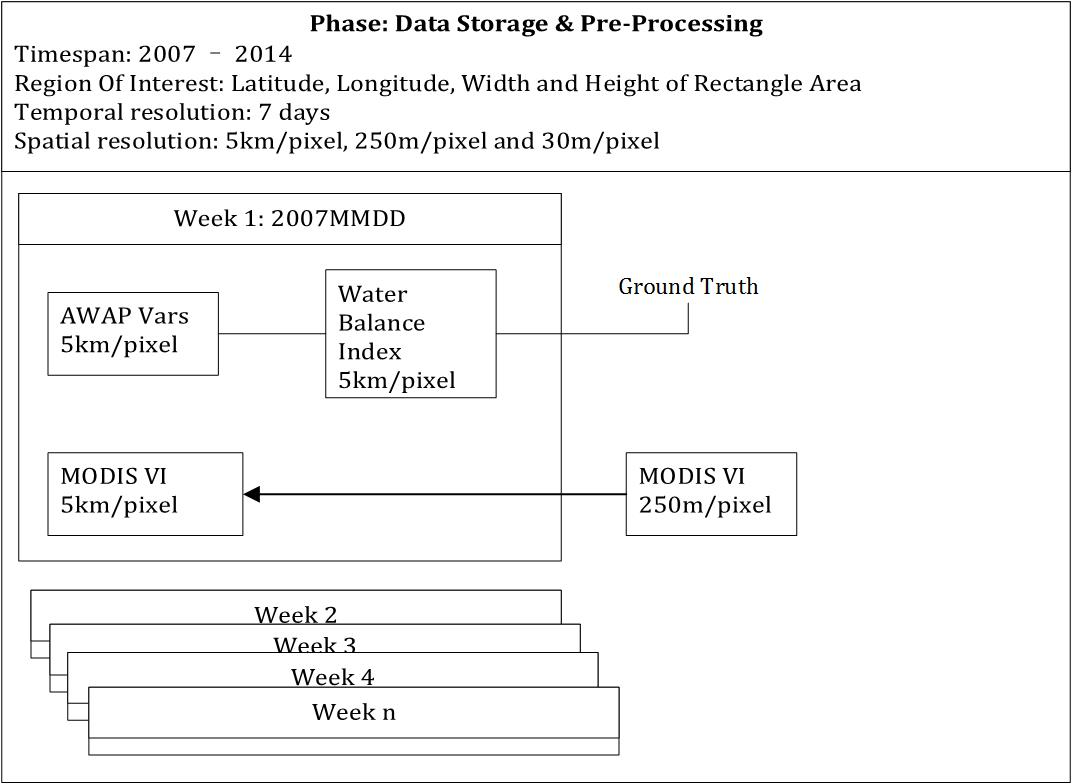
\includegraphics[width=\linewidth]{gfx/areawisephase1}
	\end{center}
	\caption{Area-wise Analysis: Data Storage \& Pre-Processing}
	\label{fig:areawisephase1}
	\end{figure}
\newline
This particular water balance model is implemented for area-wise water balance study due to its simplicity and the dependency on AWAP as the sole data source. The Java class \emph{au.csiro.iekbase.awap.WaterBalanceAWAP} implements this model, iterates through each of the extracted AWAP files and save the water balance indices in a file in the corresponding weekly folder.\\
\newline
Numerous machine learning algorithms are attempted to obtain an optimal model from the data which can be categorized into two types. Unsupervised machine learning approaches are used to understand the data, to find out whether there is certain underlying tendency and natural clusters in the data. And supervised machine learning approaches are used to explore the possibility of establishing such a model that the water balance can be estimated from VI as a proxy, using data-driven method. If successful, the water balance index can be estimated for any arbitrary region of interest at a considerably high spatial resolution which is the 250m/pixel as that of the VI data available from MODIS.
\subsection{Case study: Houston Farm}
A case study is conducted to analyze the validity and performance of proposed machine learning approaches. Data from Houston Farm (center at $42.7^\circ S, 147.5^\circ E$, rectangle width and height are both 20km), were acquired and processed as previously discussed. The time frame of interest is from year 2000 to 2014. 
\subsection{Analysis}
A total number of 320 weeks of data are filtered out among all available data sets, where for the week both AWAP and MODIS VI are successfully preprocessed and stored in the folder. For each week, the data is a matrix of size 15 by 5, where the rows are the 15 individual grids for the rectangle region of interest, and the columns are latitude, longitude, \ac{ndvi} from MODIS as input variable 1, water balance index as the output and elevation from sea level as the input variable 2, respectively. The accuracy is measured by calculating the cross-correlation of the prediction with the testing target.
\subsubsection{Approach: Neural Networks}\label{approach1}
The first attempt uses 90\% of the 320 weeks data over the 15 grids as a whole dataset to train and the rest 10\% data to test four distinct supervised learning models which are \ac{anfis}, \ac{enn}, \ac{fnn} and \ac{ffnn}. Therefore the training set contains 4320 data points, whereas the testing set contains the rest 480 data points, following the chronological order, so that the data can be learnt as a time-series.\\
\begin{quote}
\ac{fnn} was the first and the simplest type of artificial neural network devised. It has a number of layers, each subsequent layer has a connection from the previous layer, the information only moves in one direction, from the input nodes via the hidden nodes if any, to the output nodes throughout the network.\\
\newline
\ac{enn}s are FNNs with an additional layer of recurrent connections with tap delay, it is a simple algorithm for time-series modelling. \ac{ffnn} is a FNN used to fit an input-output relationship. \\
\newline
\ac{anfis} is a modelling algorithm that integrates the benefits of Fuzzy Systems and Neural Networks\citep{Jang1993}, it allows transforming human knowledge or experience into the rule base as well as providing an effective method for tuning membership functions such that the output error is minimized and/or the optimal performance is reached. It is widely used as an algorithm to model nonlinear functions and to predict chaotic time series.
\end{quote}
\autoref{table:NNanalysis1} shows the accuracy of the above four algorithms, the best performed algorithm is \ac{fnn} which has an accuracy of 21.44\%.
\begin{table}[hbt]
\caption{Algorithm Performance for \autoref{approach1}.}
\begin{center}
\rowcolors{2}{cyan!15}{white} 
\begin{tabular}{|l|l|l|l|} 
\hline
\ac{anfis}&\ac{enn}&\ac{fnn}&\ac{ffnn}\\
\hline
0.1640    &     0.1540   & 0.2144 &   0.2042\\
\hline 
\end{tabular}
\end{center}
\label{table:NNanalysis1}
\end{table}
\subsection{Approach: Neural Networks of individual grids}\label{approach2}
To improve from the previous results, an alternative way of grouping the data is used in this approach. This approach attempts to train and test each of the 15 grids individually, therefore a total of 15 best performed algorithms will be chosen to be used for estimation at later stage. Therefore the training set for each grid is 90\% of the 320 weeks data, that is 288 data points, and the testing set has 32 data points, following the chronological order.\\
\autoref{table:NNanalysis2} shows the accuracy of the four algorithms on each of the grids and the best performance out of all grids. Out of all four algorithms on Grid 15, FNN is the best performer with 62.0\% accuracy. 8 of the 15 grids have FNN as the best performed algorithm while the rest 7 have FFNN as the best performed algorithm. Neither ANFIS nor ENN scored a best performance for any of the 15 grids.
\begin{table}[hbt]
\caption{Algorithm Performance for \autoref{approach2}.}
\begin{center}
\rowcolors{2}{cyan!15}{white} 
\begin{tabular}{|l|l|l|l|l|c|} 
\hline
&\ac{anfis}&\ac{enn}&\ac{fnn}&\ac{ffnn}&Best Performer\\
\hline
Grid 1& 0.2352& 0&0.4058&0.3273&FNN\\ \hline
Grid 2&0.0567&0.0595&0.2571&0.2200&FNN\\ \hline
Grid 3&0.3058&0.3079&0.3314&0.3286&FNN\\ \hline
Grid 4&0.3022&0.3708&0.3717&0.2963&FNN\\ \hline
Grid 5&0.3427&0.3102&0.4567&0.5625&FFNN\\ \hline
Grid 6&0.4250&0.1888&0.5001&0.4736&FNN\\ \hline
Grid 7&0.3449&0.2450&0.3812&0.5321&FFNN\\ \hline
Grid 8&0.3914&0.1235&0.4865&0.5635&FFNN\\ \hline
Grid 9&0.3720&0.1111&0.4085&0.4697&FFNN\\ \hline
Grid 10&0.2438&0.1531&0.4401&0.4064&FNN\\ \hline
Grid 11&0.2938& 0&0.2469&0.3758&FFNN\\ \hline
Grid 12&0.3845& 0&0.4959&0.5207&FFNN\\ \hline
Grid 13&0.3589&0.1869&0.2461&0.4536&FFNN\\ \hline
Grid 14&0.3059&0.3228&0.3781&0.3568&FNN\\ \hline
Grid 15&0.5816&0.0393&0.6200&0.5811&FNN\\ \hline 
\end{tabular}
\end{center}
\label{table:NNanalysis2}
\end{table}
\subsubsection{Surface Estimation}\label{WBestimate}
One application of this supervised learning approach is to enhance the spatial resolution of the water balance indices for the given area of interest, which is originally at 5km/pixel as it is calculated from AWAP data that is of the same resolution. With successfully trained and tested models which take inputs from MODIS VI and outputs from water balance indices, a surface map that is of the same resolution (250m/pixel) as the MODIS VI, the input data, can be estimated. The enhanced water balance surface map for the Houston farm case study is shown in \autoref{fig:wbsurface}. However, the generated enhanced map has inconsistent coloring in terms of variation and strength for each of the grids, as well as poor inter-grid transitions.
\begin{figure}[hbt]
\myfloatalign 
\subfloat[{Water Balance Surface, each grid using a distinct model.}]
{\label{fig:WBestimate2D}
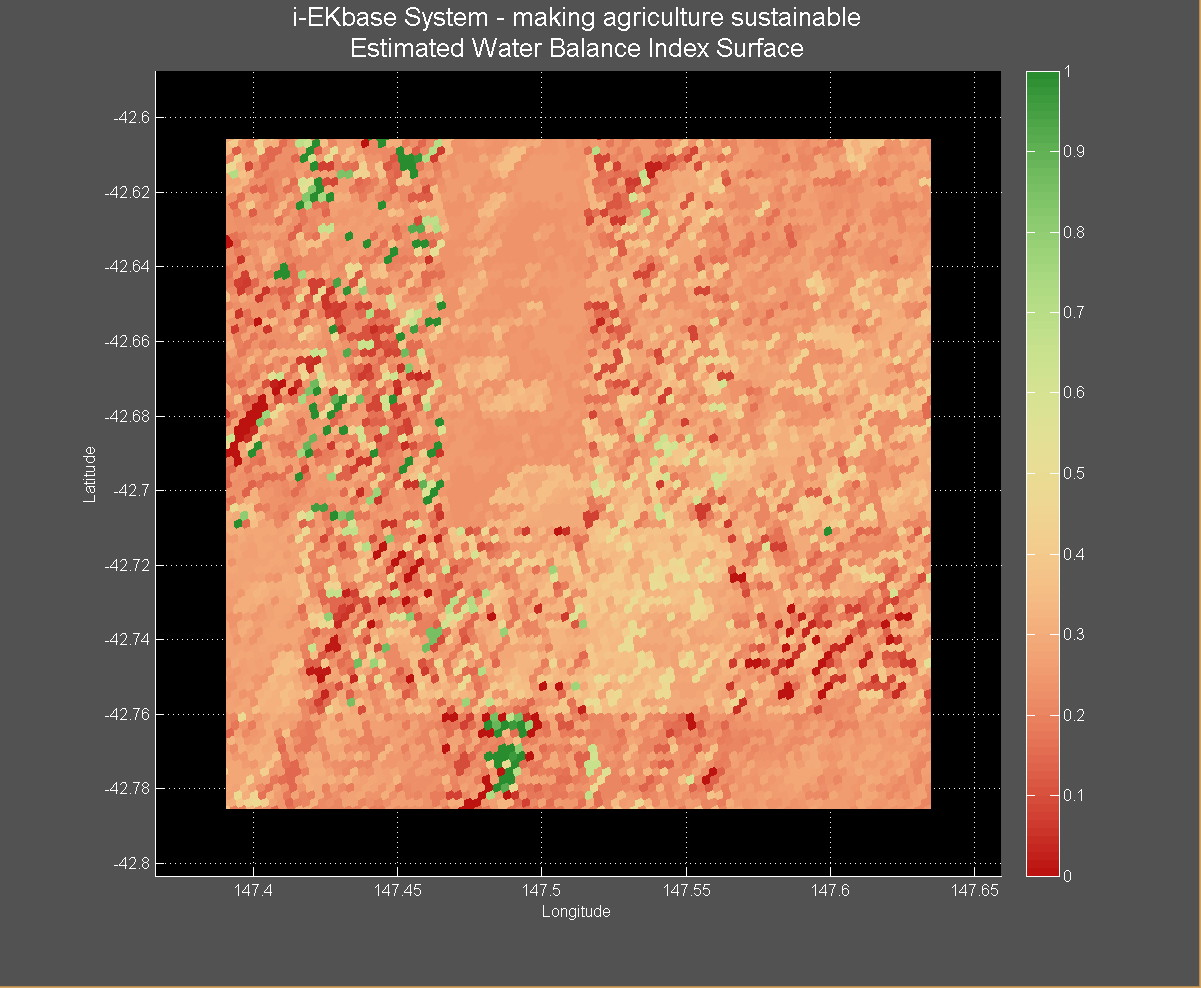
\includegraphics[width=.45\linewidth]{gfx/WBestimate2D}} \quad
\subfloat[{Water Balance Surface in 3D. Z data: elevation. Pixel color: Water Balance Index.}] 
{\label{fig:WBestimate}
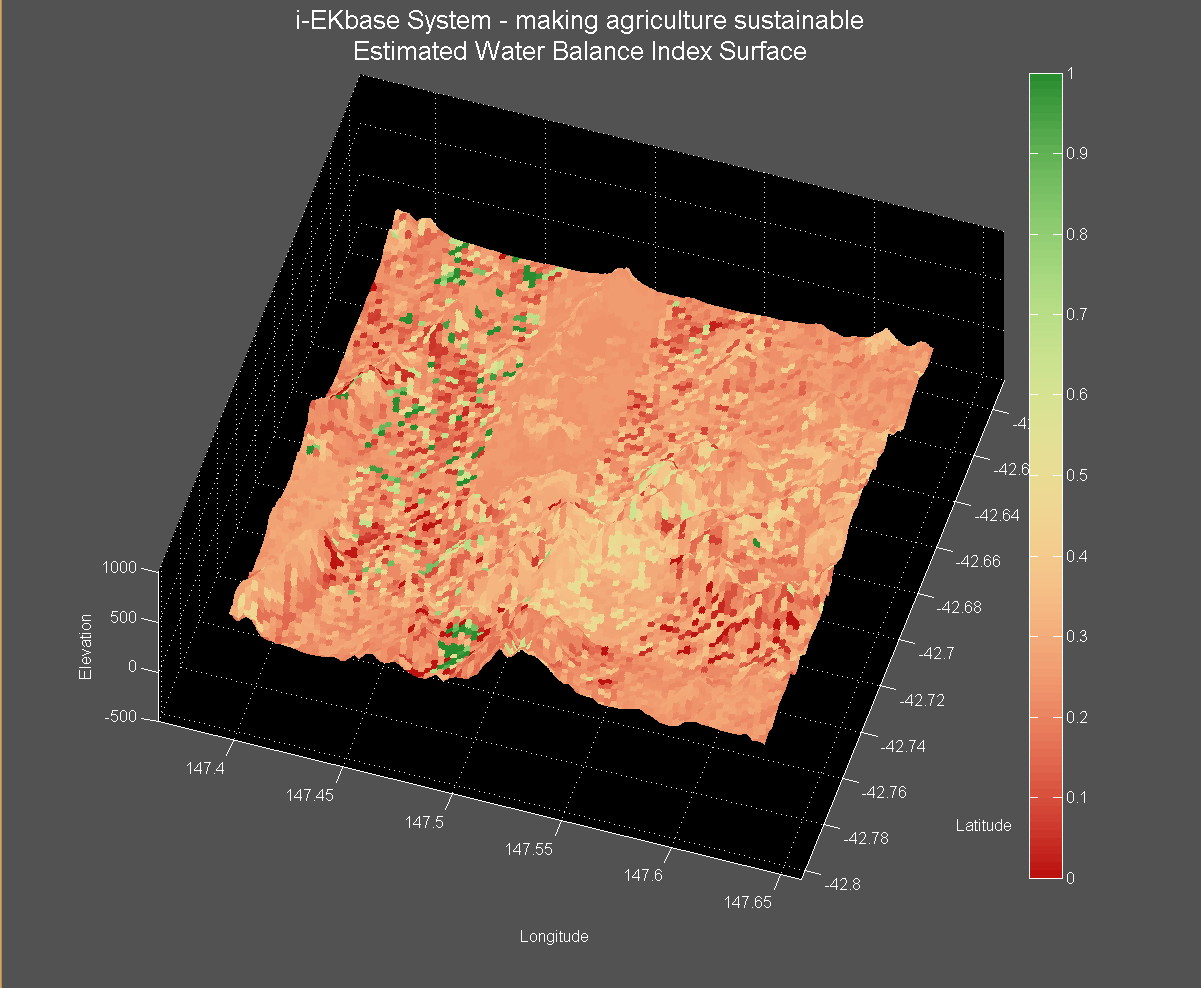
\includegraphics[width=.45\linewidth]{gfx/WBestimate}} 
\caption{Enhanced water balance surface for Houston farm using neural network algorithms}
\label{fig:wbsurface}
\end{figure}
\subsection{Approach: Ensemble Classification}\label{approach3}
This approach regards the entire 320 weeks 15 grids data as a collection of independent points, with input of MODIS VI, and output of water balance index calculated from AWAP data. In contrary to the previous two supervised approaches where the data are kept in a chronological order, in this approach the data are randomized to avoid any bias introduced by chronological information, e.g. seasonal changes etc. Also, the output values are classified into n intervals, such that there is at least 1 output data in each of the interval.\\
\newline
The ensemble classification is a supervised learning approach that construct a set of various classifiers and combine them to classify test data by averaging. It is well-accepted that ensemble approach has a superior performance than individual classifiers that constitutes as the base for the ensemble\citep{Kim2003}\citep{Dietterich2000}. Five different ensemble classification algorithms are used for this analysis which can perform classification with three or more classes, namely Bagging Tree, AdaBoost Tree, RUSBoost Tree, Subspace Discriminant and Subspace K-Nearest-Neighbour.\\
\newline
\autoref{table:ENanalysis} contains the experiment results of different trials that use increasing number of classes. Where
\begin{quote}
Accuracy = (True Positives + True Negatives)/(Positives + Negatives)\\
Sensitivity = True Positives/(True Positives + False Negatives)\\
Specificity = True Negatives/(False Positves + True Negatives)
\end{quote}
The result has improved from previous approaches, for the first trial with 10 classes, the best performed algorithm RUSBoost has an accuracy of 66.18\% which is higher than the best result from \label{approach2}. The accuracy of the best performed algorithm converges to a maximum of 92.06\% as the number of classes reaches to the maximum possible of 53 which is due to the constraint that there must be at least 1 element in each of the evenly spaced intervals. \autoref{fig:WBestimateTS} plots the estimated water balance time series using the best performed algorithm and the ground truth time series for the grid of coordinate $42.6057^\circ S, 147.3903^\circ E$.
\begin{table}[hbt]
\caption{Algorithm Performance for \autoref{approach3}.}
\begin{center}
\rowcolors{2}{cyan!15}{white} 
\begin{tabular}{|l|l|l|l|l|l|} 
\hline
No. of Classes&Best Performer&Accuracy&Sensitivity&Specificity\\
\hline
10&RUSBoost& 0.6618&0.2323   & 0.8025 \\ \hline
20& RUSBoost& 0.7998 &   0.1149  &  0.9227 \\ \hline
30&RUSBoost&0.8625  & NaN&    0.96086\\ \hline
40&RUSBoost&0.9010 &  NaN  &   0.9994  \\ \hline
50&RUSBoost& 0.9201 &      NaN &   0.9995\\ \hline
53&RUSBoost&0.9206    &   NaN   & 0.9992    \\ \hline
\end{tabular}
\end{center}
\label{table:ENanalysis}
\end{table}
	\begin{figure}[hbt] 
	\begin{center}
	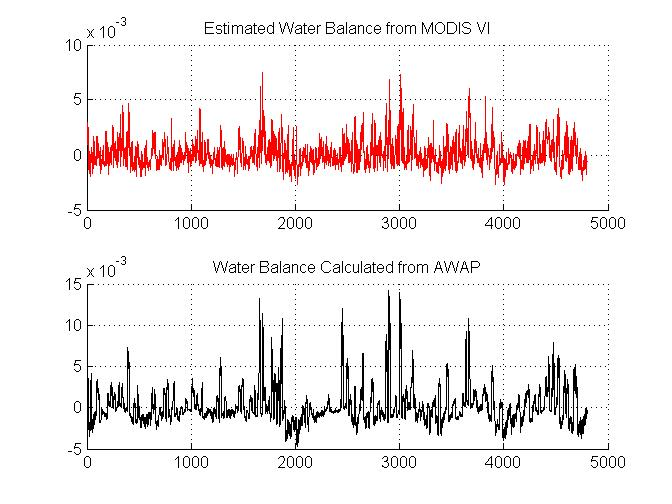
\includegraphics[width=.95\linewidth]{gfx/WBestimateTS}
	\end{center}
	\caption{Estimation vs. Ground Truth}
	\label{fig:WBestimateTS}
	\end{figure}
\subsubsection{Surface Estimation}
Similar to \autoref{WBestimate}, an enhanced water balance surface is generated for the Houston farm case study, using 50 evenly spaced classes and RUSBoost algorithm, trained and tested with randomized data, which has an accuracy of 92.01\%. The surface plot is shown in \autoref{fig:wbsurface2}.
\begin{figure}[hbt]
\myfloatalign 
\subfloat[{Water Balance Surface, using RUSBoost Ensemble Classification with 50 classes.}]
{\label{fig:WBestimate2D_2}
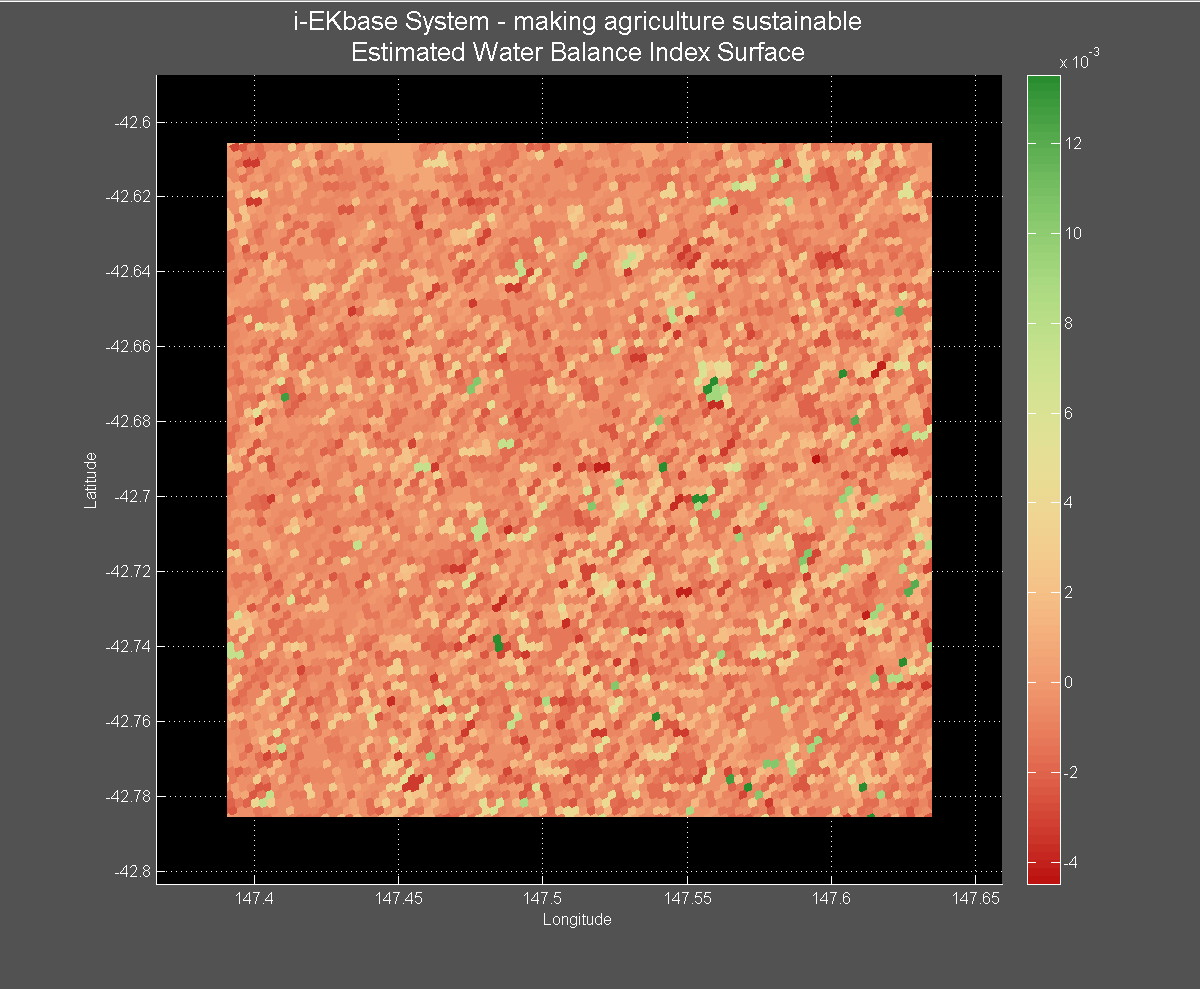
\includegraphics[width=.45\linewidth]{gfx/WBestimate2D_2}} \quad
\subfloat[{Water Balance Surface in 3D. Z data: elevation. Pixel color: Water Balance Index.}] 
{\label{fig:WBestimate_2}
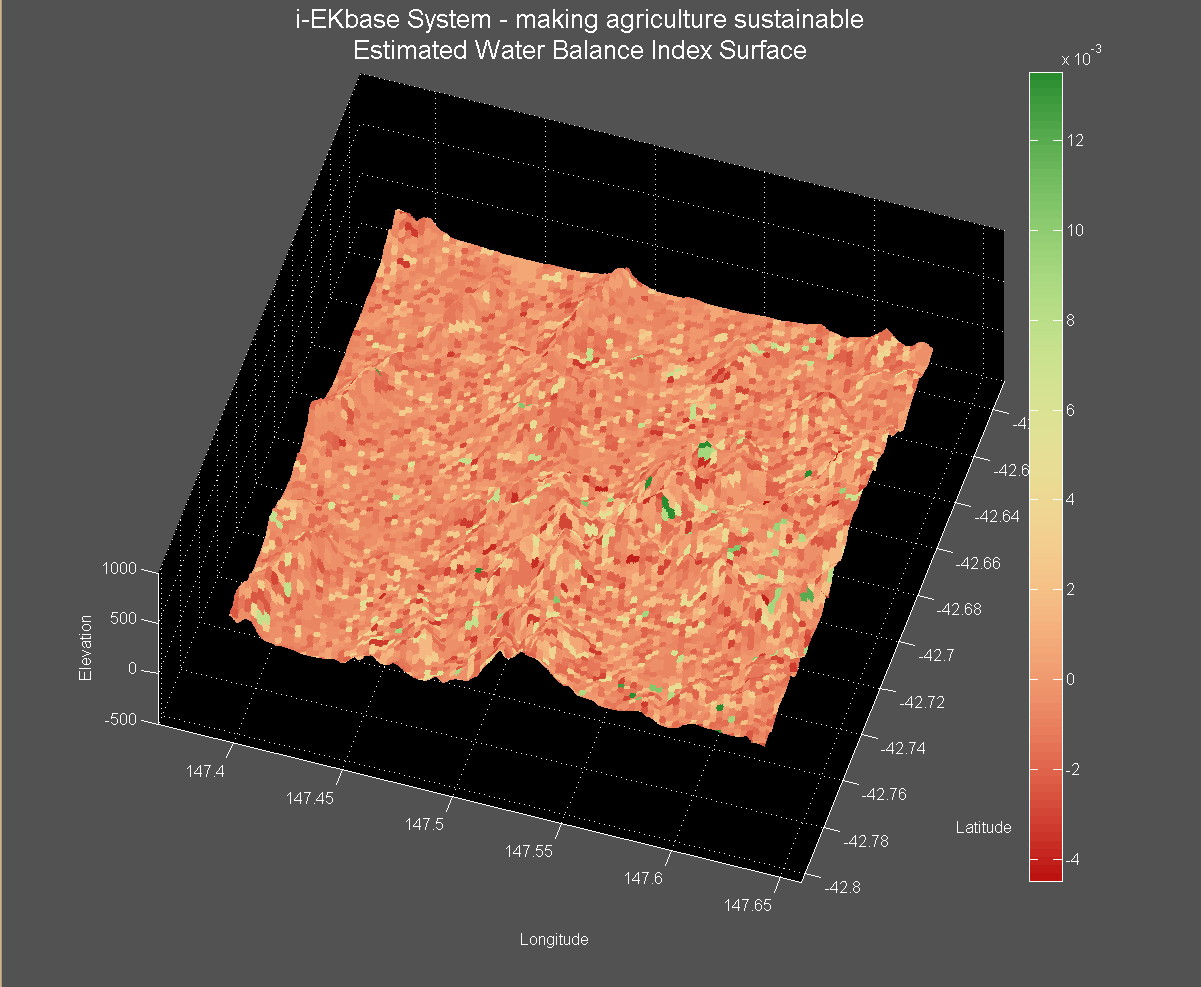
\includegraphics[width=.45\linewidth]{gfx/WBestimate_2}} 
\caption{Enhanced water balance surface for Houston farm using ensemble classification algorithms}
\label{fig:wbsurface2} 
\end{figure}
\subsection{Interpretation of Results}
Three algorithms are attempted for the area-wise study of the data, and the results have improved progressively through each of the stage. The ensemble classification algorithm has the best performance with a maximum accuracy of 92.06\%. Upon further cross-validation of this result, it means that the model and approach explained in the thesis is proven to be valid, that is, MODIS VI of resolution 250m/pixel can be used as a proxy for the water balance index derived from AWAP data. Therefore, given any point that has MODIS VI data available, it is valid to estimate the water balance index for that point. In fact, this has been succeeded and shown in the previous section where an enhanced resolution water balance surface is generated via this method, which is beyond the capability of the conventional approach where only AWAP data is used. In addition, this approach is more credible than an cubic interpolation algorithm which is often used to enhance spatial resolution.